\chapter{Environment and context}\label{chap:context}

\begin{sectionIntro}
    This chapter will describe essential facts about my internship, such as
    which company I did my internship in and what I worked on.
\end{sectionIntro}

\section{Company}

\subsection{Celad}
Celad is an IT consulting company with about 800 employees. It was created in Toulouse
and its headquarters are still in Toulouse.
The major activities of Celad cover:
\begin{description}
    \item [Information systems] such as solutions for E-banking, E-business, mobile applications.
    \item [Embedded sector] such as real-time, electronics, and aerospace.
\end{description}
One of its biggest clients in the embedded sector in Toulouse is Intel.
I did my internship as a contractor for Intel via Celad.

\subsection{Intel}
Intel Corporation is the world’s largest semiconductor chip maker. They
introduced the first microprocessor in 1971 and have been the world leader in
silicon innovation since.
Following a strategy to extend the Intel Architecture to new market segments,
they are delivering smartphones and tablets powered by Intel chipsets.

On figure \ref{fig:razri} below there is a picture of a smartphone with Intel inside.

\begin{figureGraphics}{Motorola Razr I with Intel inside}{fig:razri}
    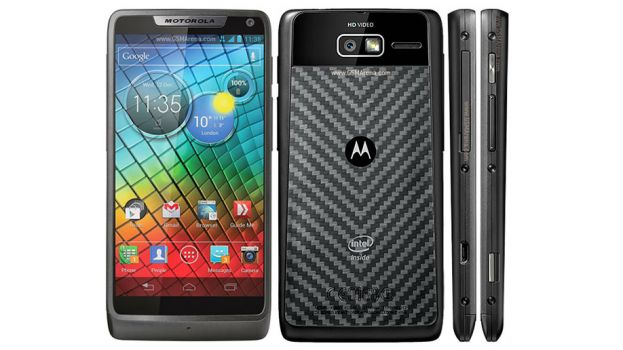
\includegraphics[width=\textwidth]{./src/img/razri.jpg}
\end{figureGraphics}

Some key figures of Intel:
\begin{itemize}
\item Leading manufacturer of computer, networking and communications
  products,
  \item 300 Facilities in 50 countries,
  \item Over \$35B in Annual Revenues from customers in over 120
    countries,
\item 23 Consecutive years of positive net income,
\item Approximately 80,000 employees,
\item 43,000 technical degrees, 12,000 Masters in Science, 4,000
  PhD’s, 4,000 MBA’s,
  \item One of the top ten most valuable brands in the world for 10
    consecutive years,
\item Invests \$100 Million each year in education across more than 50
  countries,
\item One of the top ten Linux \gls{kernel} contributors.
\end{itemize}

\subsection{Intel Audio feature team in Toulouse}
The team I worked with is the Audio feature team, in Toulouse.
They are responsible for the Audio \gls{hal} which is the interface between the
\gls{android} layers and the \gls{kernel}. Intel made a custom Audio \gls{hal} to
replace \gls{android} default's one with their own one, which provides more features.
The Intel Audio \gls{hal} is present in every \gls{android} device from 2011 or later with Intel inside, such
as the \emph{Motorola Razr I} from figure \ref{fig:razri} which has an Atom processor.

Their custom \gls{hal} is based around the \gls{pfw}, which will be described in the section \ref{sec:parameter-framework}.


\section{Topic of my internship}
I worked within the Intel Audio development team, as an \emph{agile
software developer}. The team is customer oriented, using \gls{scrum}
methodology (see chapter \ref{chap:organisation}). My tasks
within the team were focused around open-sourcing the \gls{pfw} on
\gls{GitHub}\footnote{the links are in the annex at page \pageref{chap:annex}}


\subsection{Why open-sourcing the Parameter-framework}\label{sec:whyOpensourcing}
At the moment there is no standardization (such as POSIX for operating systems) in middleware. Due to the lack
of standards, each company is reinventing their own solution for handling middleware problems in their own way.
The \gls{pfw} which is the solution developed by the Intel Audio team is \emph{generic}, \emph{efficient} and \emph{scalable} enough to become a standard.
With this ambition in mind, the Intel Audio team decided to open-source the core component of their Audio \gls{hal}, the \gls{pfw}.
The component is hosted on \gls{GitHub} which is the most popular code hosting site in the world.

\subsection{My role regarding open-sourcing}
In order to open-source such a complex component as the \gls{pfw}, the Intel Audio team needed to evaluate if the code was ready.
The code requires to be easy-to-understand so that the open-source community is willing to adopt it.
Since I had never worked with that component before, I took a fresh look at the code. I had to try to \emph{understand the code} and the
\emph{concepts} (explained at section \ref{sec:parameter-framework}) of the \gls{pfw} without any documentation.

At the same time, internal developments were also made on this component, but on a different version of it.
This implies that there are two code repositories of the same component: the \emph{internal} one and the \emph{open-source} one.
Keeping the two code repositories synchronized is very important because each divergence has a huge maintenance impact.
My role was to setup and execute that synchronization process to avoid costly and painful future maintenance.
How this was done will be detailed later in section \ref{sec:syncProcess}.



\section{Android}
During my internship, I worked on the \gls{android} platform. This operating
system has a complex software stack which goes from the Linux \gls{kernel} to
applications such as \emph{Gmail}. This section gives an overview of the Android
stack in order to highlight the part I worked on.

\subsection{Global Android architecture}
Android is a complex system, having more than 1 billion active users.
It is structured in different levels:

\begin{description}
    \item[Applications] such as Gmail, which are seen by the end-user
    \item[Applications Framework] which is used by the applications, this is written in Java.
    \item[Libraries] which is composed of the Dalvik virtual machine and other C/\gls{cpp} frameworks.
    \item[Hardware Abstraction Layer] which a part of the middleware stack that ties together the libraries
        and the \gls{kernel}. I worked in this section of the \gls{android} stack.
    \item[Linux kernel] which contains the drivers and provides the user-space functionalities for the
        middleware stack.
\end{description}

The figure \ref{fig:archi} shows android software stack and highlights the
part I worked on during my internship, which is the Audio \gls{hal}.

\begin{figureGraphics}{Global Android architecture}{fig:archi}
    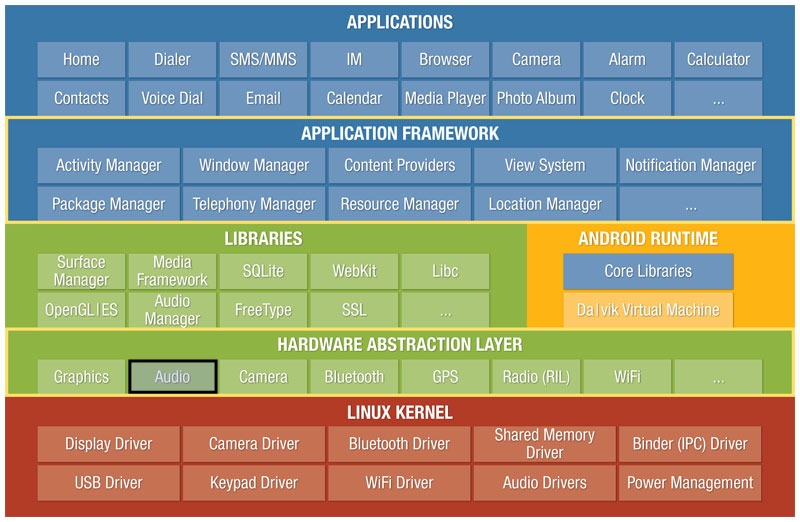
\includegraphics[width=\textwidth]{./src/img/android-archi-audio-hal.jpeg}
\end{figureGraphics}

The Audio \gls{hal} is also one of the primary concerns of the Audio team in Toulouse and will be detailed
in next section


\subsection{Intel Audio HAL}
Intel's Audio \gls{hal} for Android platforms is based on a generic, plugin-based solution: the \gls{pfw}.
It runs in the \emph{userland}, which is easier to maintain than kernel-space code. This is due
to the fact that we can use more high level languages such as \gls{cpp}.
Since this solution is plugin-based, it is easy to extend and add more subsystems if needed.

There is an overview of the Intel Audio \gls{hal} on figure \ref{fig:hal} below.
\begin{figureGraphics}{Simplified view of Intel Audio HAL}{fig:hal}
    \includegraphics[height=0.5\textheight]{./src/img/hal-architecture.pdf}
\end{figureGraphics}
Two different instances of \gls{pfw} exist in the Intel Audio \gls{hal}:
\begin{description}
    \item[The route Parameter-framework] communicates with the \emph{Stream Manager} and the \emph{Route Manager}.
        This side is responsible for translating events which come from upper layers into \emph{routes}, which
        is the concept understandable by the route manager.
    \item[The audio Parameter-framework] communicates with the \emph{Route Manager} and the \gls{alsa} driver.
        This side talks to the drivers in order to set the different mixers in the correct state. For example,
        changing the gain of a mixer.
\end{description}

Some requirements of the Intel Audio \gls{hal}:
\begin{itemize}
    \item Since the audio system needs to be tuned by the tuning engineers, the \gls{hal} should be configurable.
        It would have been very painful to recompile the code at each time it is needed to adapt the value of a mixer!
    \item Since the \gls{hal} needs to \emph{abstract} the hardware variations, it should also be scalable. It should be
        easy to support new hardware.
\end{itemize}

The \gls{pfw} is a way to fulfill those requirements.


\section{Parameter-framework}
\label{sec:parameter-framework}
In this section we will have an overview of the \gls{pfw}, which is the core component of my internship.

The \gls{pfw} is a plugin-based and rule-based framework for handling parameters.
It allows you to describe \emph{what} parameters we want to control given the means to explain \emph{how} to access
them and \emph{when} to change their settings.
Figure \ref{fig:pfwContext} illustrates that.

\begin{figureGraphics}{Three questions the Parameter-framework answers}{fig:pfwContext}
    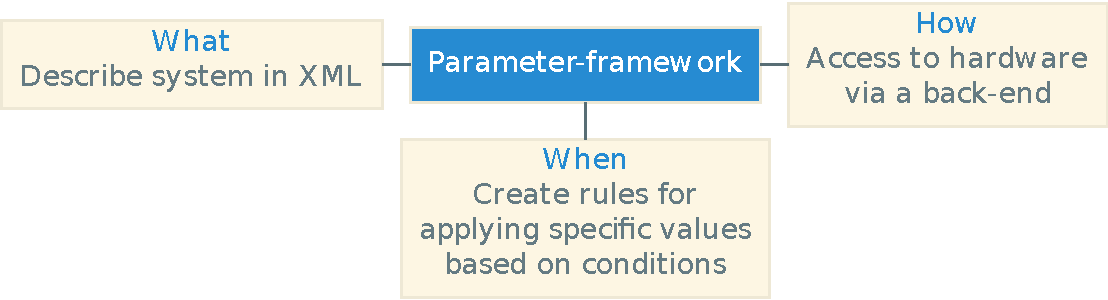
\includegraphics[width=\textwidth]{../presentation/src/img/pfwContext.pdf}
\end{figureGraphics}

This means that you can:
\begin{itemize}
    \item Describe your system's structure and its parameters (in \gls{xml}) - aka. \emph{What}
    \item Write (in \gls{cpp}) or reuse a backend (aka. plugin) for accessing the parameters that you just described - aka. \emph{How} (Structure)
    \item Define (in \gls{xml} or in a domain-specific-language) conditions/rules upon which a given parameter must take a given value - aka. \emph{When} (Settings)
\end{itemize}

With this concepts, we can cover all the requirements we have for creating a scalable \gls{hal}.
Now we are going to have a look at the motivation behind the creation of this framework.

\subsection{Motivation}
During a phone call, the smartphone isn't just transmitting the sound received from the microphone. Various algorithms are
applied on the audio signal which is transmitted and received.
Figure \ref{fig:audioArch} below shows an example of an audio architecture which shows the components involved.

\begin{figureGraphics}{Simplified audio architecture of a pandaboard}{fig:audioArch}
    \includegraphics[width=\textwidth]{./src/img/audio-architecture.pdf}
\end{figureGraphics}

The sound goes:
\begin{itemize}
    \item Trough the \emph{voice modem}
    \item Via the \emph{Audio DSP} where some voice processing algorithms (such as noise reduction) are applied
    \item Towards the \emph{codec} to send the audio signal to the headset.
\end{itemize}

Those algorithms have a lot of parameters, which can change depending on the accessory for e.g. whether we are using a headset,
or using the speaker. Furthermore, those parameters are \emph{often hardware dependent}.

The \gls{pfw} was designed to manage easily those multiple parameters in a scalable way.

\subsection{Some concepts}
In this section we are going to discover the concepts that make the
\gls{pfw} such a powerful tool.

\subsubsection{Structure}
The \gls{pfw} is first of all a hierarchical tree of parameters.
On figure \ref{fig:pfwtree} we can see an example of audio tree.

\begin{figureGraphics}{Parameter framework tree example}{fig:pfwtree}
    \fbox{\begin{minipage}{6cm}
            \dirtree{%
                .1 audio.
                    .2 microphone.
                        .3 echo\_cancellation.
                            .4 enable.
                            .4 configuration.
                                .5 gain.
                                .5 coefficient.
                    .2 speaker.
                        .3 equalizer.
                            .4 enable.
                            .4 configuration.
                                .5 filter.
                                .5 coefficient.
            }
    \end{minipage}}
\end{figureGraphics}

These structures are stored in \gls{xml} files. This is great because it implies that we don't need
to recompile the \gls{pfw} when changing the structure we are describing.

In listing \ref{lst:pfwstructure}, when can see the \gls{xml} structure file
describing the tree from figure \ref{fig:pfwtree}.

\begin{code}[language=pfwXml, caption=Structure file example snippet, label=lst:pfwstructure]
<!--snippet-->
<ComponentType Name="echo_cancellation">
    <BooleanParameter Name="enable"/>
    <ParameterBlock Name="configuration">
        <IntegerParameter Name="gain" Size="8"/>
        <IntegerParameter Name="coefficient" Size="8"/>
    </ParameterBlock>
</ComponentType>
<!--snippet-->
\end{code}

\subsubsection{Settings}
The \gls{pfw} is also able to change multiple parameters without any manual action, depending on the context.
The context is defined using a set of criteria. Those criteria are variables which can take a set of defined values.
For example, a criterion called \emph{Input Device} can take several values such as \emph{Microphone} or \emph{Headset}.

Depending on the value of those criteria, the \gls{pfw} can automatically apply a set of values towards
multiple parameters.
On listing \ref{lst:pfwsettings} we can see an example of setting file, written in a special language
which is translated into \gls{xml} by our build system.

\begin{code}[language=pfwLang, caption=Settings file example, label=lst:pfwsettings]
Domain:
    Conf: SpeakerWithEchoCancel
        InputDevice Is Microphone
        Component: audio/speaker/
            echo_cancellation/enable = true
            configuration/gain = 2
            configuration/coefficient = 3
        # -- snippet --
    Conf: HeadsetWithEchoCancel
        InputDevice Is Headset
        Component: audio/headset/
            echo_cancellation/enable = true
            configuration/gain = 3
            configuration/coefficient = 4 # arbitrary values
        # -- snippet --
\end{code}

\subsubsection{Extensibility}
Since the \gls{pfw} is \emph{plugin-based}, it is easy to extend its functionality to other usages than Audio, such
as Camera, or Bluetooth. I contributed on the filesystem plugin for example, which can be used to handle \lstinline{/proc/} entries.
